\section{Implementation of Neural Network in CLAS12 software}

The models described in earlier stages were implemented in the tracking code of CLAS12 
software. 


\subsection{Track Identification Workflow}

 Track identification consists of two parts programmed to be done in two passes.
First, all clusters reconstructed by the clustering algorithm are grouped into sectors and super-layers.
In the first pass over the data signals from each sector of drift chambers are analyzed to create a track 
candidate list consisting of 6 segments.
The resulting track candidates are evaluated by the classifier neural network to assign a probability to each 
of the candidate being either positive or negative track. The list of track candidates is sorted by probability and the list is passed
to another algorithm that is responsible for removing tracks that have lower probability of being a "good" track and have
clusters that they share with a "good" track candidate with higher probability. In this procedure the first track from 
the list is taken (which already has the highest probability of being a "good" track since list is sorted) and then the program
iterates over the track candidates starting from position number 2 and to the end of the list and removes all tracks that share a 
cluster with the track at position 1. Then track candidate at position 1 is moved from the track candidate list into the identified
track list. Then the iteration starts again, and the procedure is repeated until there are no track candidates left in the list.

 \begin{figure}[!h]
\begin{center}
 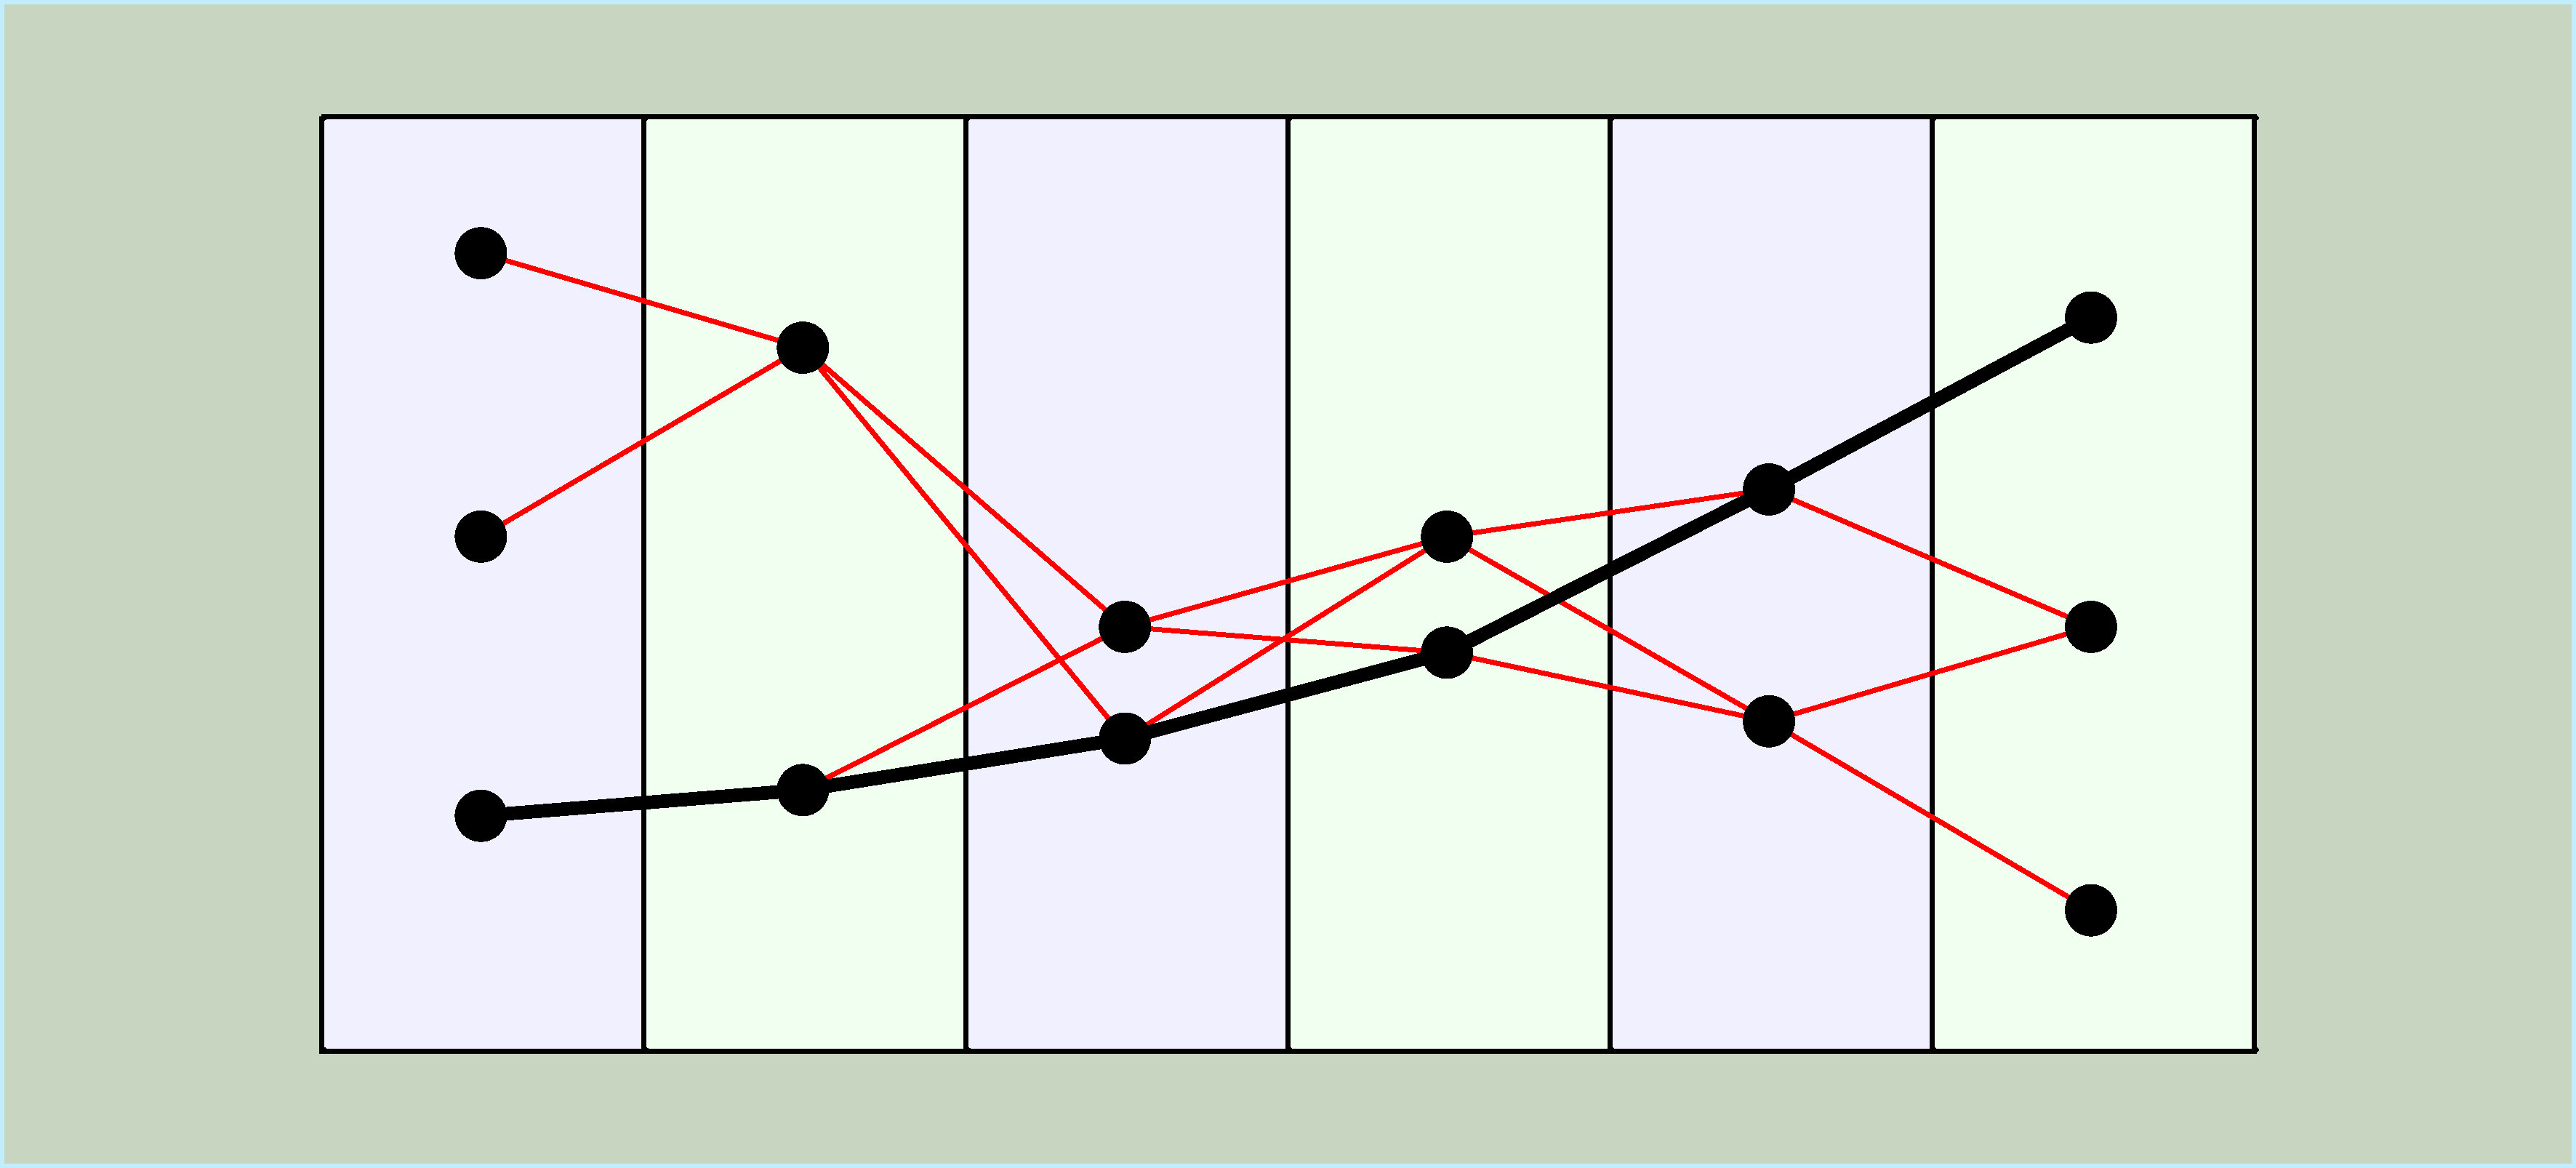
\includegraphics[angle=90,width=1.2in]{images/iden_6_sl.pdf}
  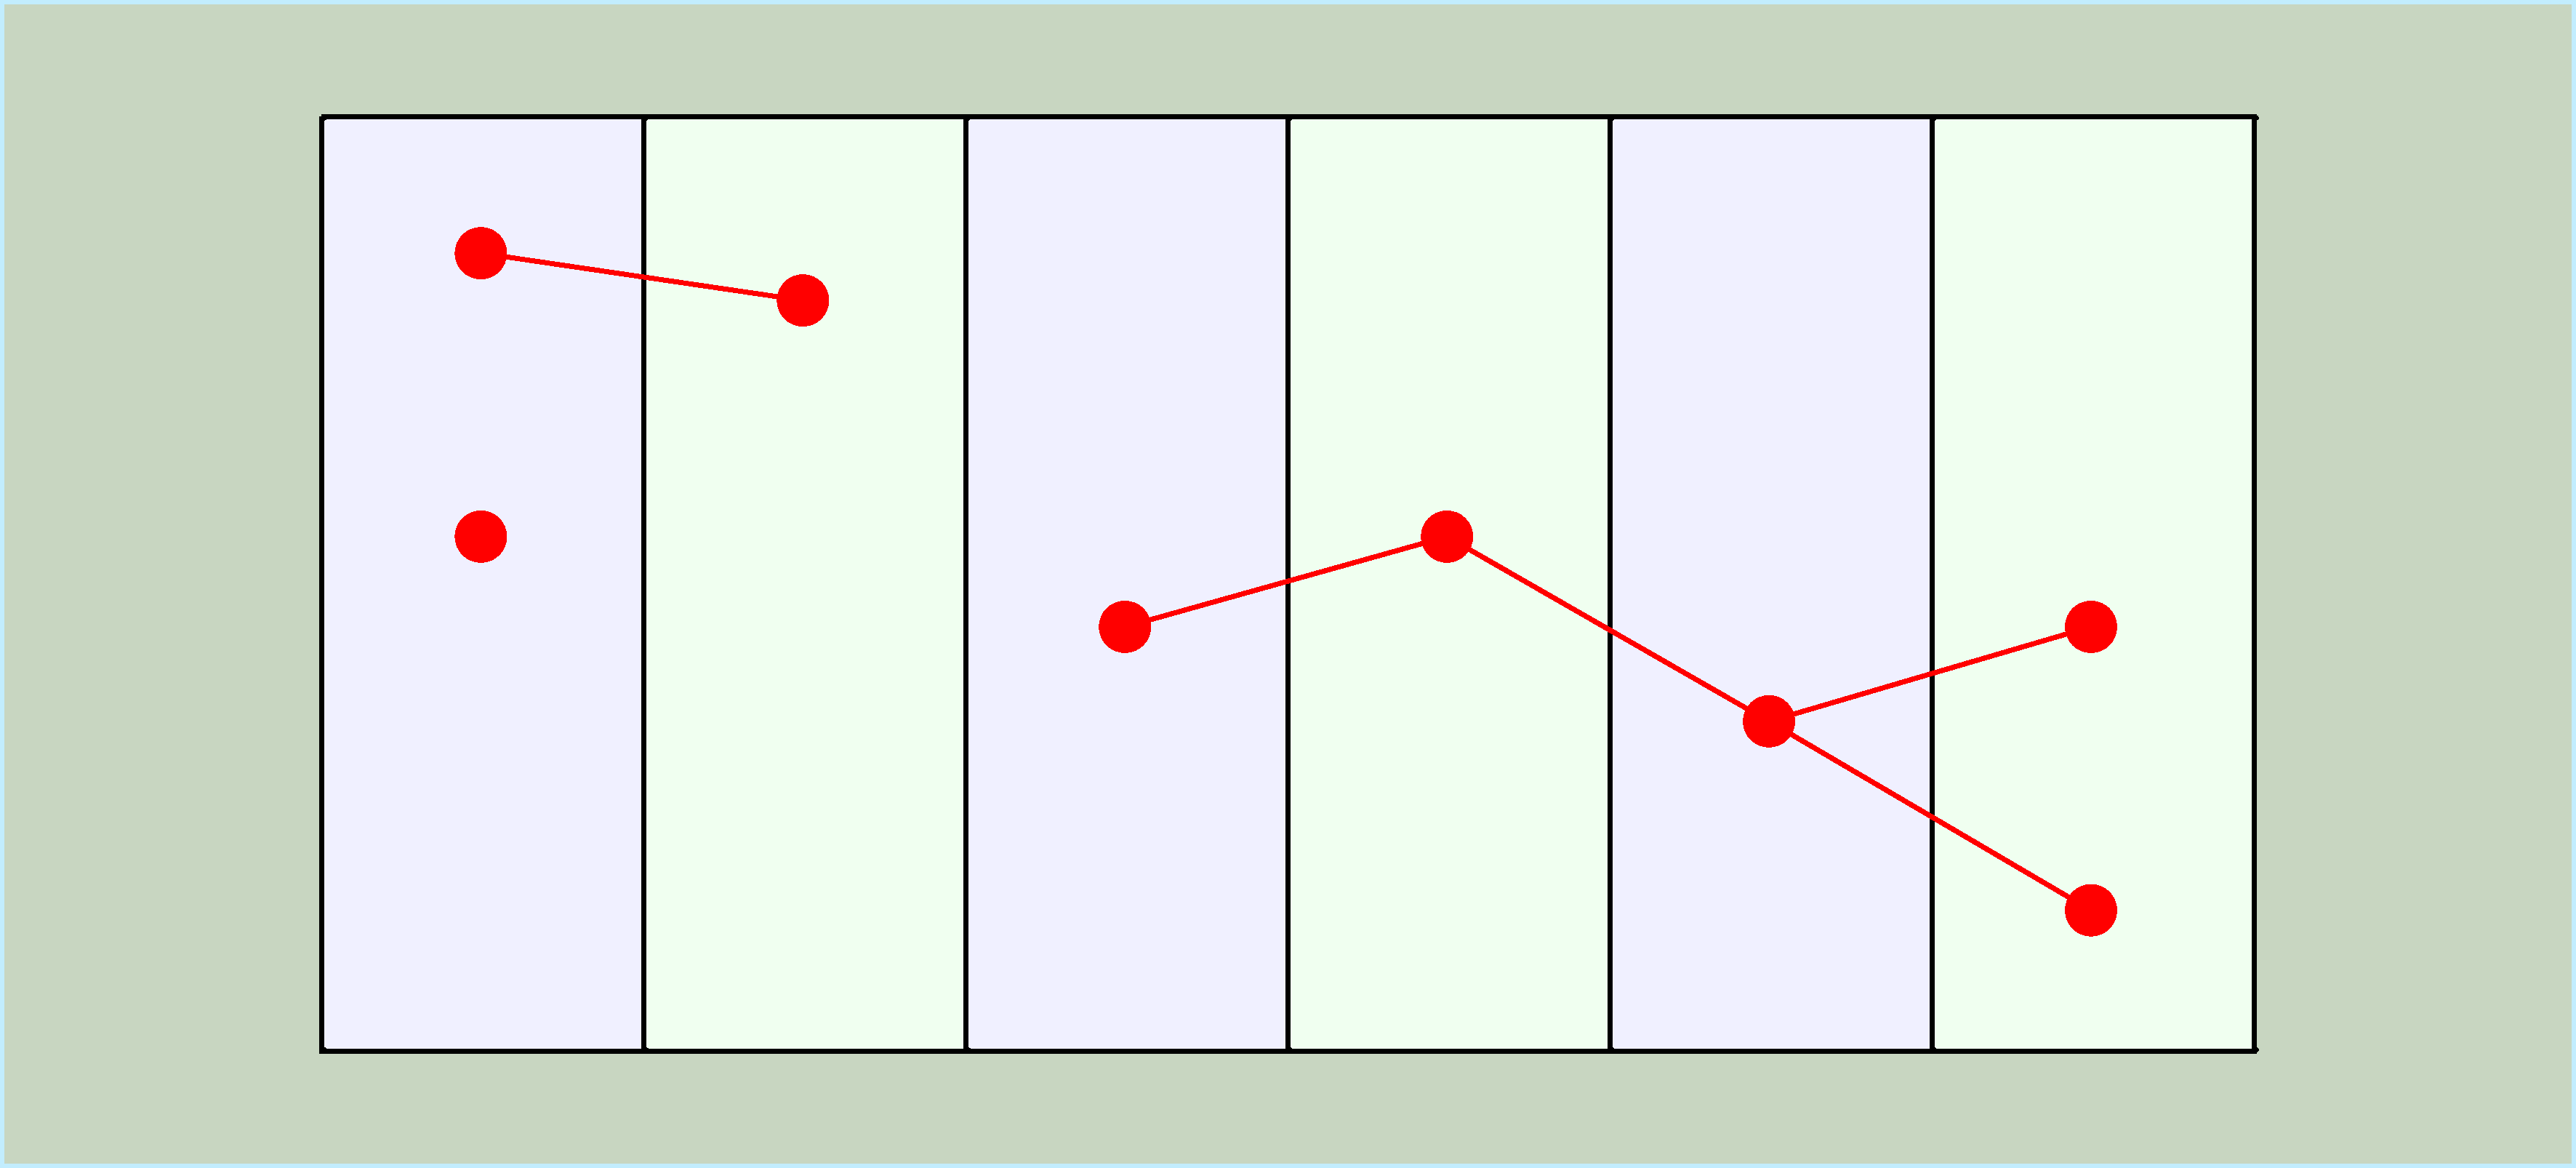
\includegraphics[angle=90,width=1.2in]{images/iden_5_sl_a.pdf}
    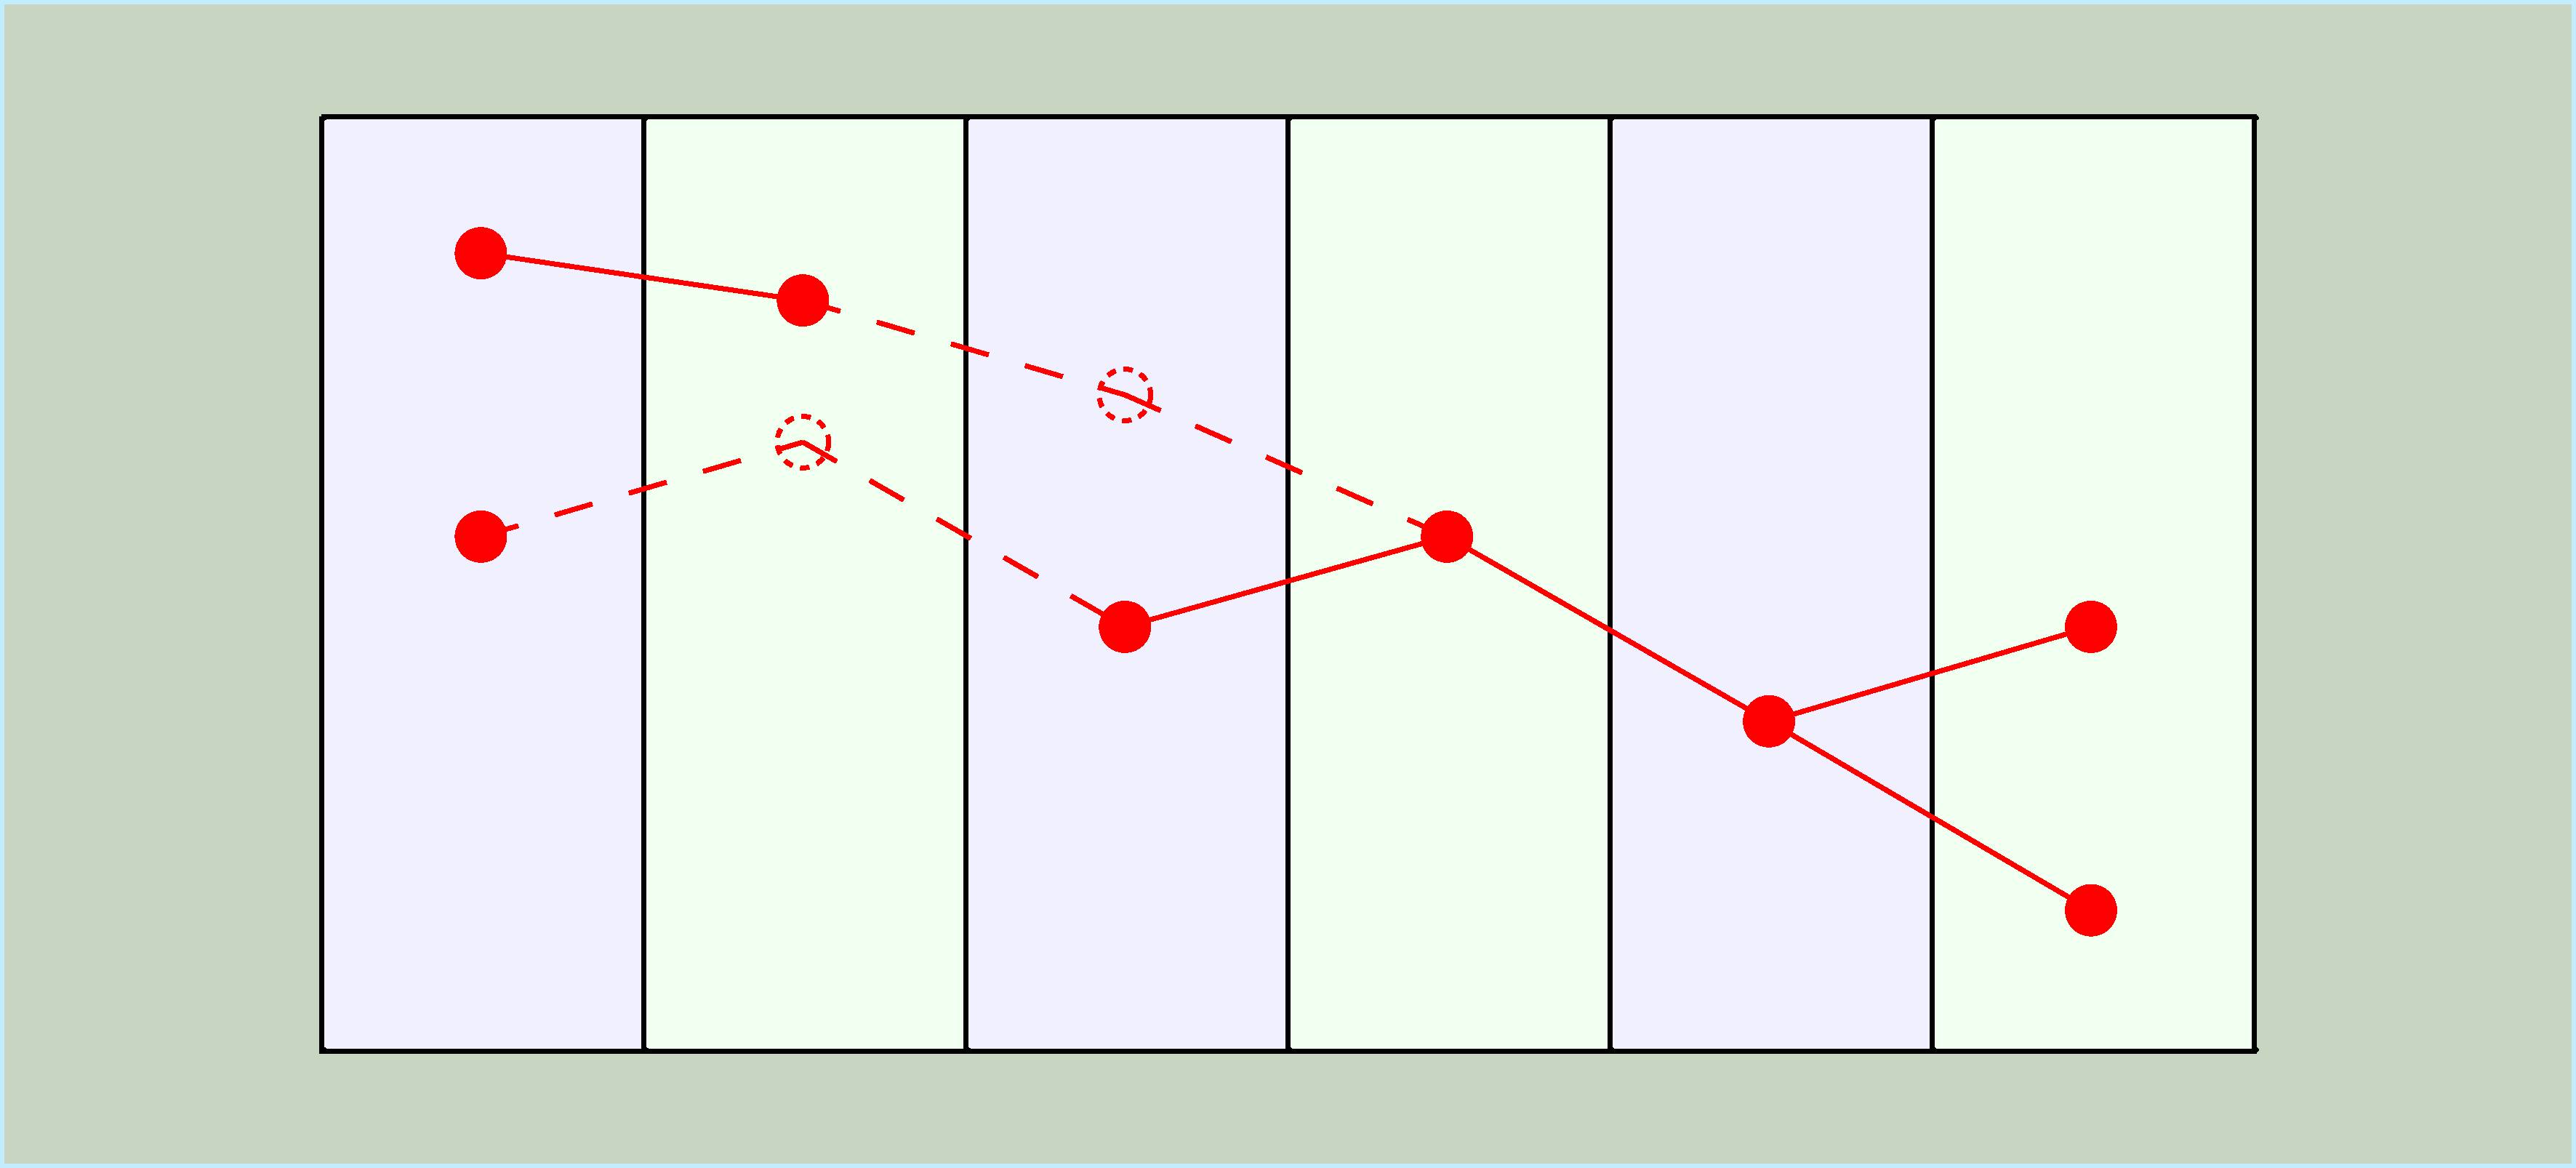
\includegraphics[angle=90,width=1.2in]{images/iden_5_sl_b.pdf}
      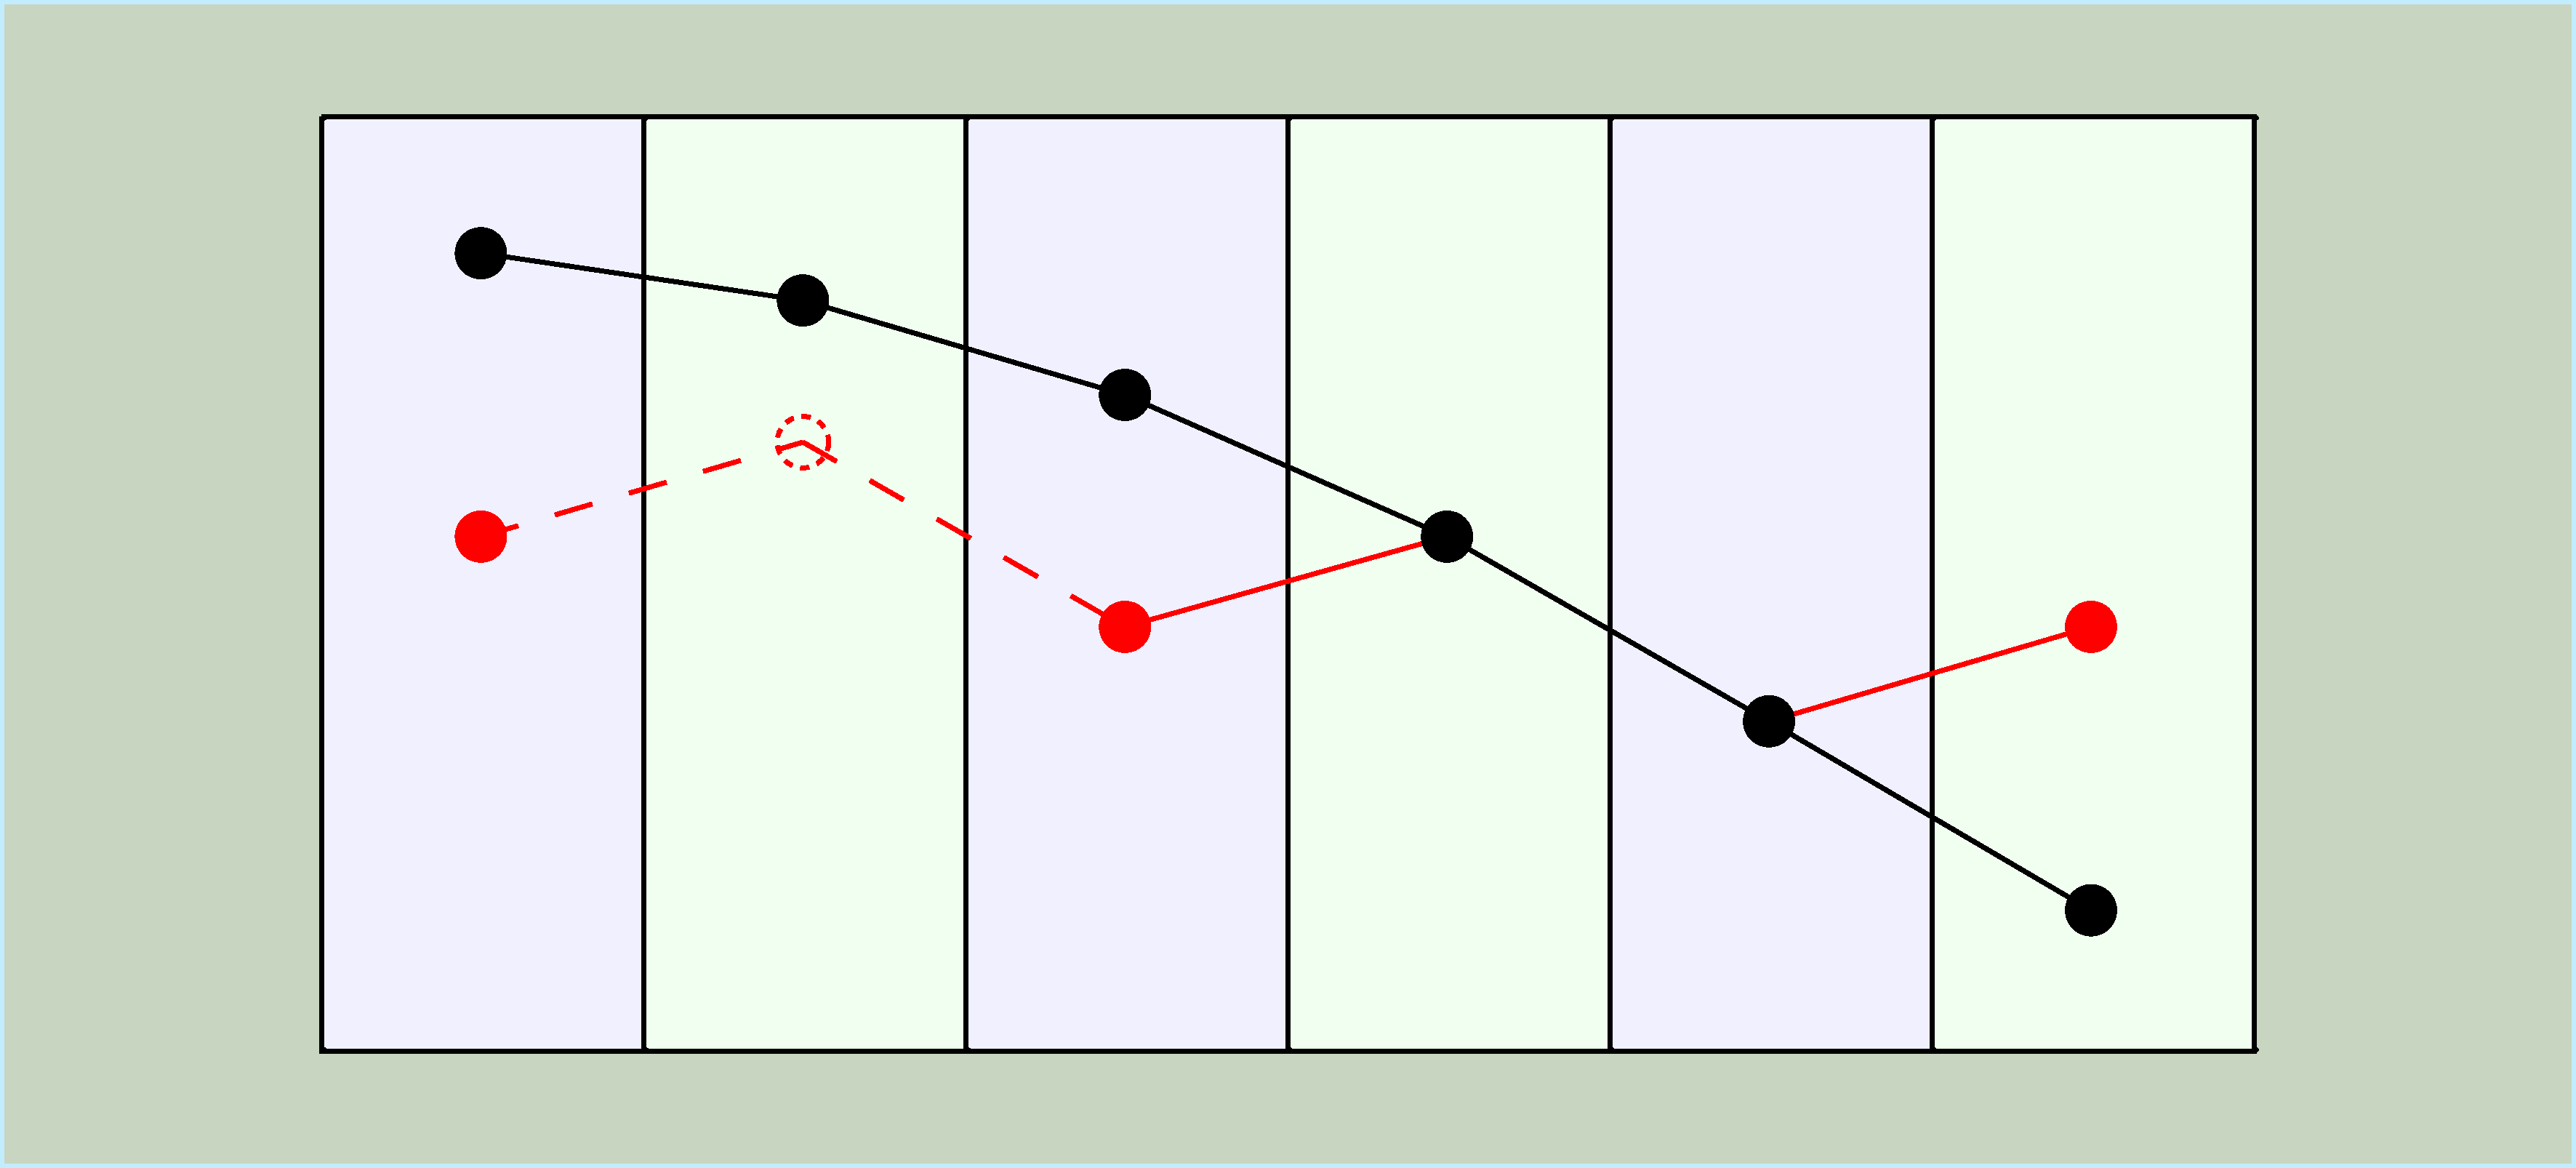
\includegraphics[angle=90,width=1.2in]{images/iden_5_sl_c.pdf}
            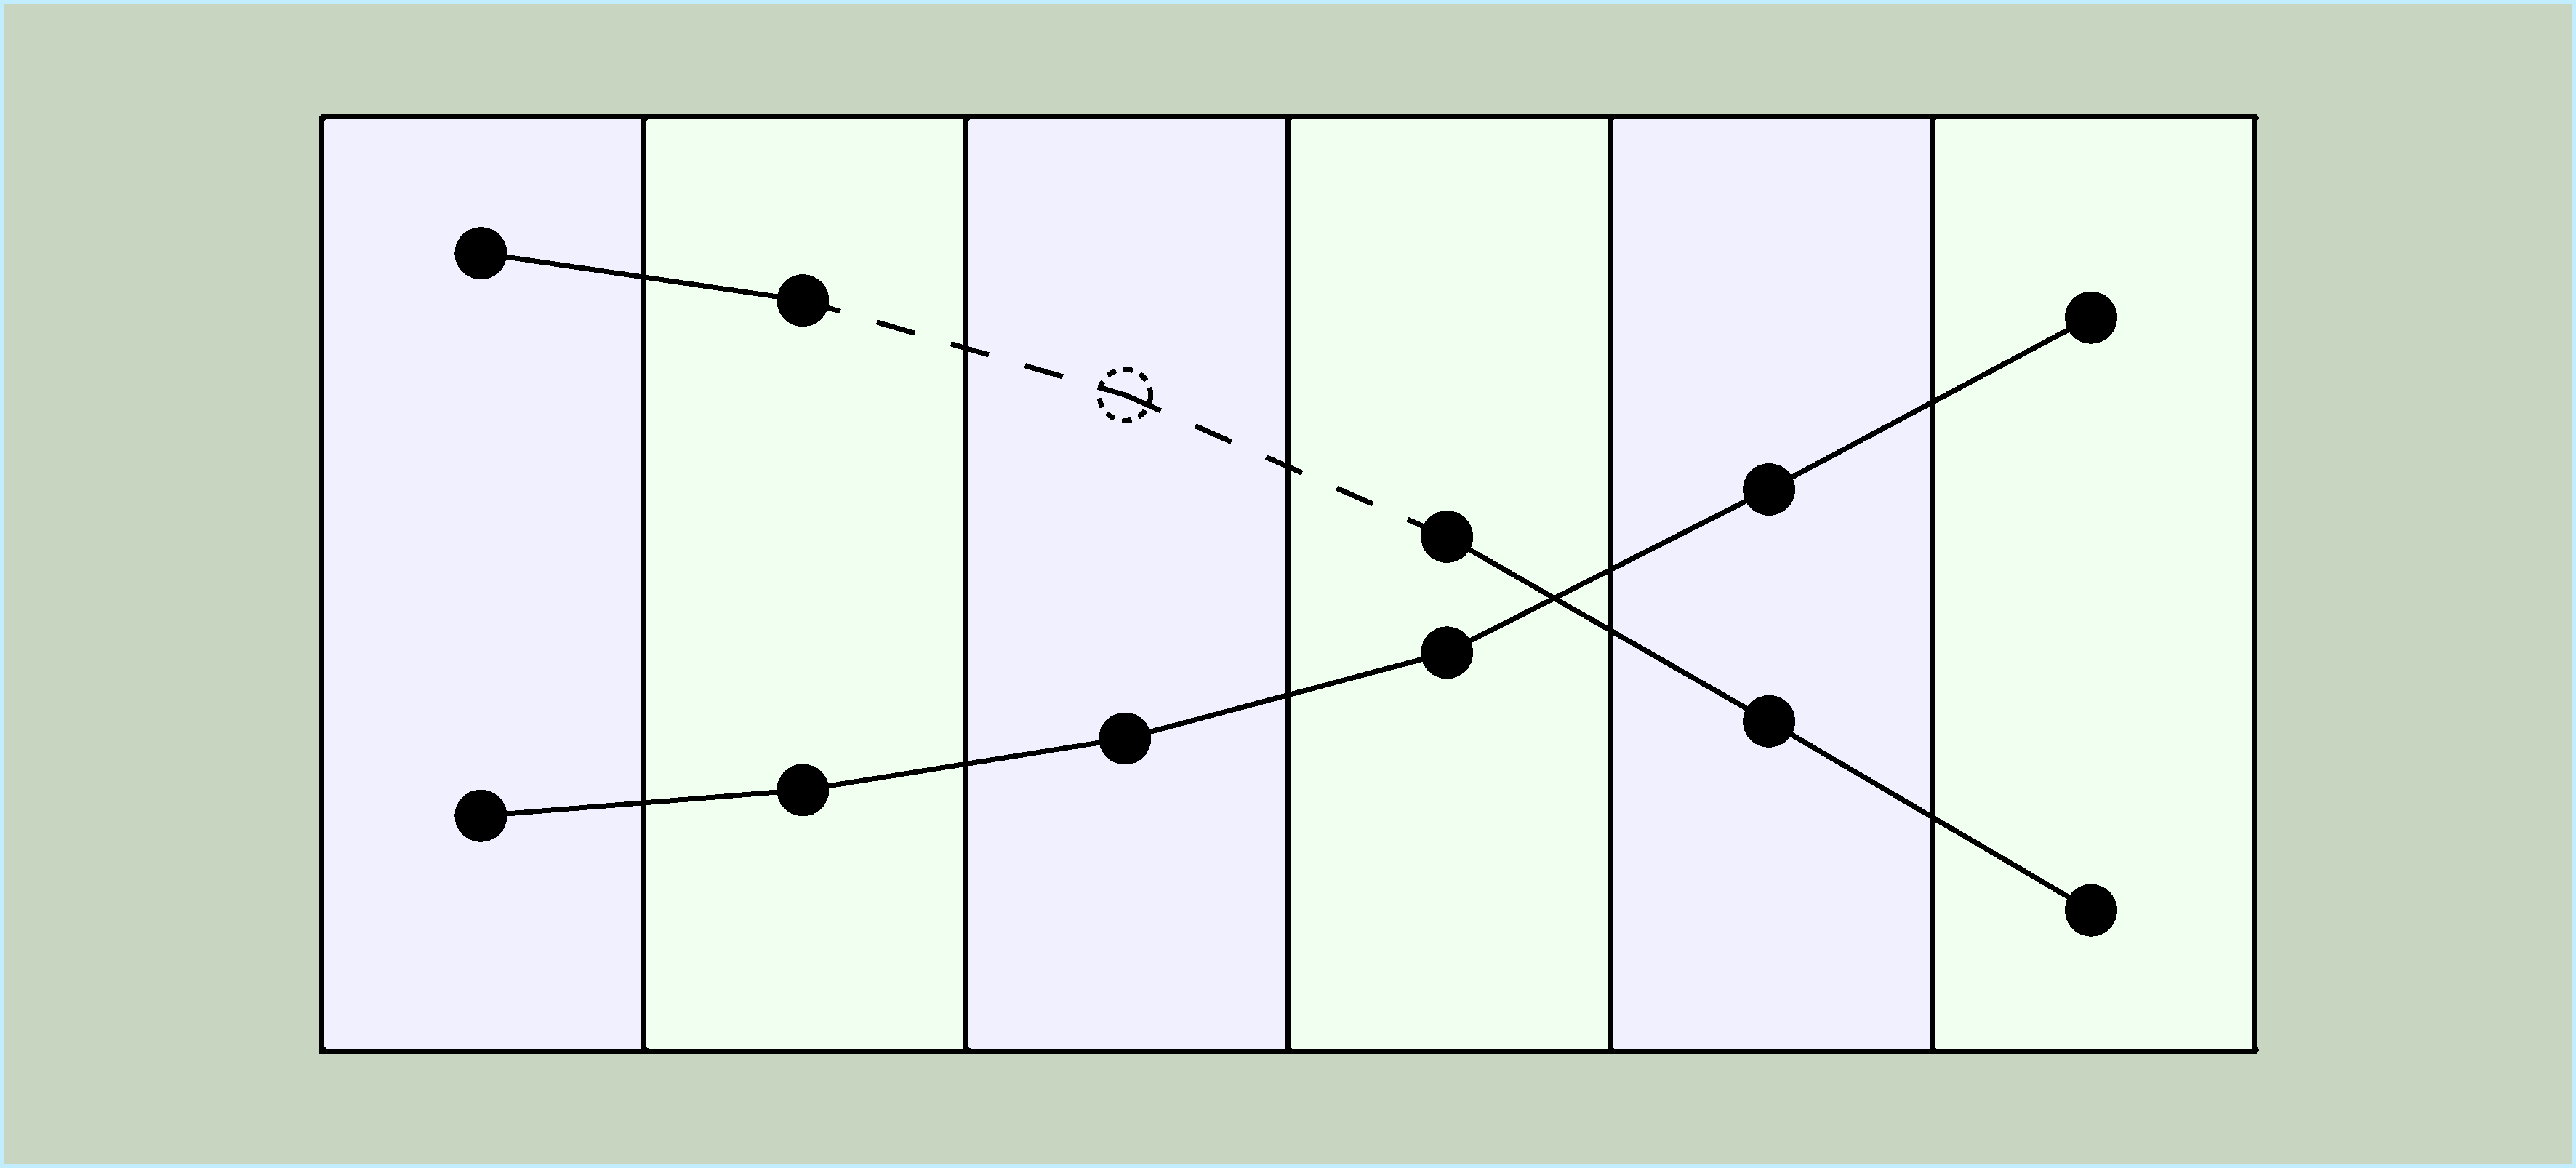
\includegraphics[angle=90,width=1.2in]{images/iden_5_sl_d.pdf}

\caption {Stages of Neural Network track identification procedure. 1) identifying 6 super-layer tracks. 2) removing all hits 
belonging to a identified track and constructing 5 super-layer track candidates. 3) generating pseudo-clusters for 5 super-layer
track candidates using corruption fixing auto-encoder. 4) identify good track candidates from the list of 6 super-layer 
(one of the super-layers is pseudo-cluster) track candidates. 5) isolate both identifies (6 super-layer and 5 super-layer) tracks 
for further fitting with Kalman-Filter.}
 \label{network:procedure}
 \end{center}
\end{figure}

The second stage of track identification starts by constructing a list of track candidates with combinations of 5 clusters 
out of 6 from all existing clusters (one per super-layer). Then all track candidates that have a shared cluster with tracks
identified at the first stage of classification are removed from the list. After this, for each track candidate with a missing cluster
in one of the super-layers, a pseudo-cluster is generated using the Corruption Auto-Encoder Network and the missing super-layer 
cluster is assigned the inferred value, hence turning all track candidates to 6 cluster track candidates. Then, the 
cured (or fixed) track candidate list is passed to the track classifier module described above, which evaluates the list with
the classifier neural network and isolates tracks with the highest probability of being good track. 

\subsection{Implementation in reconstruction software}

The CLAS12 reconstruction software framework is a Service Oriented Architecture platform (CLARA \cite{Gyurjyan:2011zz}).
The reconstruction software consists of several microservices, each responsible for processing data from one
detector \cite{Ziegler:2020gsr}. The reconstruction procedure for some of the detector components can also 
be broken down into smaller logical microservices to add some flexibility in changing the implementation of the small parts, 
and provide alternative reconstruction procedures for some of the components.
Reconstruction of tracks in drift chambers is a complex task and consists of several parts.
The first stage of the process is to isolate clusters
from the hits in drift chambers (called clustering service). Once the clusters are isolated, track candidates are formed from all combinations 
of 6 segments. The track candidates are analyzed to determine which good candidates from remaining segment 
combinations of 5 segment tracks are constructed which are also fitted to determine which ones are potential good tracks.
The later module (hit based tracking) determines good track candidates based only on hit positions of the track candidates (no timing
informations is used at this level). At the later stages of the tracking code (time based tracking), chosen good track candidates are further refined with the Kalman filter by using timing information from each of the sensors (drift chamber wires). By the time the reconstruction code reaches the time based tracking stage, the track candidates are already defined. 

\begin{figure}[!ht]
\begin{center}
 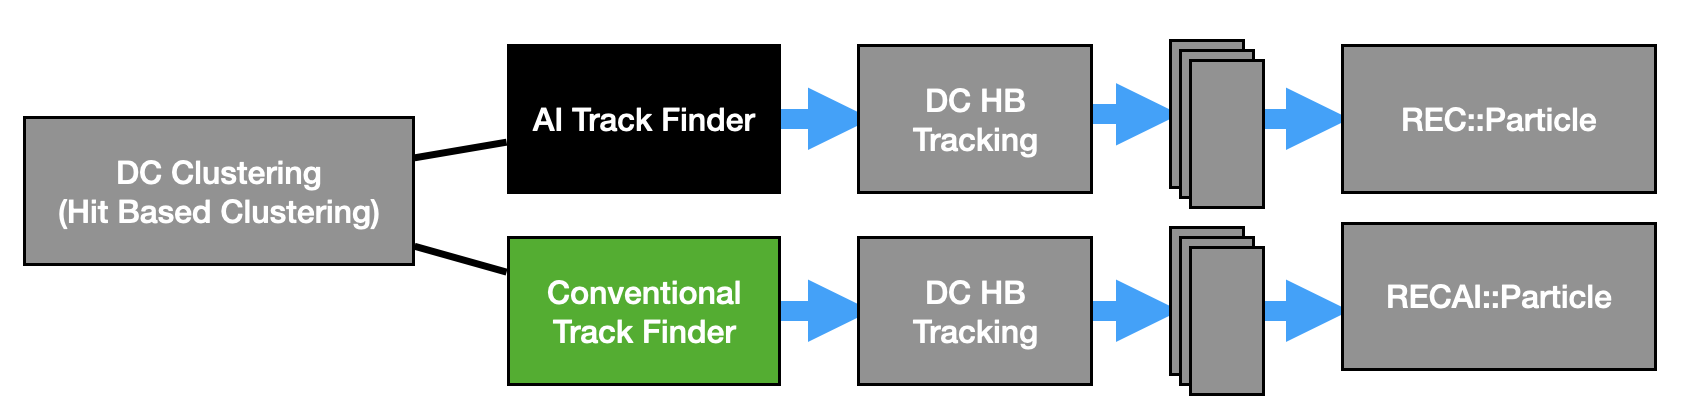
\includegraphics[width=6.0in]{images/recon_diagram.png}
\caption {Diagram of reconstruction workflow with Artificial Intelligence included. Tracking software splits into two parallel branches : one where reconstruction is done by the conventional algorithm, and one where only tracks isolated by AI are fitted by Kalman filter.}
 \label{recon:diagram}
 \end{center}
\end{figure}

In order to implement our neural network into the reconstruction workflow we designed two parallel branches in the reconstruction code where we run 
two algorithms to identify good tracks from track candidate lists, one based on the conventional algorithm and a second based on the neural network.
Both algorithms store their track suggestions in separate data structures, and pass them to the next stage where track parameters are reconstructed by 
conventional tracking algorithm using Kalman filter. This approach lets us have two parallel outputs from the tracking code in order to compare the performance of
each method.

